\documentclass[conference]{IEEEtran}
\IEEEoverridecommandlockouts
% The preceding line is only needed to identify funding in the first footnote. If that is unneeded, please comment it out.
\usepackage{amsmath,amsthm,amssymb} %modos matemáticos y  simbolos
\usepackage{latexsym,amsfonts} %simbolos matematicos
\usepackage{cancel} %hacer la linea que cancela las ecuaciones
\usepackage[spanish, es-noshorthands]{babel} %comandos en español y cambia el cuadro por la tabla
\decimalpoint %cambia las comas por puntos decimal
\usepackage[utf8]{inputenc} %caracteristicas del español
\usepackage{physics} %Simbolos fisicos
\usepackage{array} %mejores formatos de tabla
\parindent =0cm %sangria 
\usepackage{algorithmic}
\usepackage{graphicx}
\usepackage{textcomp}
\usepackage{xcolor}
\usepackage{mathtools} 
\usepackage[framemethod=TikZ]{mdframed}%Entornos talegas
\usepackage[colorlinks = true,
			linkcolor = blue,
			citecolor = black,
			urlcolor = blue]{hyperref}%formato de los links y URL's
\usepackage{multicol} %varias columnas
\usepackage{enumerate} %enumeraciones
\usepackage{pgf,tikz,pgfplots} %documentos en formato tikz
\usepackage{mathrsfs} %letras chingonas (transformada de laplace)
\usepackage{subfigure} %varias figuras seguidas
\usepackage{tabulary}
\usepackage{multirow} %ocupar varias filas en una tabla
\usepackage{fancybox} %recuadros talegas
\usepackage{float} %ubicar graficas
\usepackage{color}
\usepackage{comment}
\usepackage{stackrel}
\usepackage{calligra}
\usepackage{lipsum}
\usepackage{cite}
%\pgfplotsset{compat=1.17} 

\newcommand{\R}{\mathbb{R}}
\newcommand{\Z}{\mathbb{Z}}
%%%%%%%%%%%%%%%%%%%%%%%%%%%%%%%%%%%%%%%%%%%%%%%%%%%%%%
\def\BibTeX{{\rm B\kern-.05em{\sc i\kern-.025em b}\kern-.08em
    T\kern-.1667em\lower.7ex\hbox{E}\kern-.125emX}}
\begin{document}



%%% CARÁTULA
\begin{titlepage}



\begin{flushleft}
    Universidad de San Carlos de Guatemala \\
    Escuela de Ciencias Físicas y Matemáticas \\
    Curso: Laboratorio de Instrumentación \\
    Profesor: Wendy Miranda
\end{flushleft}

\vspace{8cm}

\begin{center}
    \huge{Parcial 1}
\end{center}

\vspace{10cm}

\begin{flushright}
    Diego Sarceño \\
    $201900109$
\end{flushright}

\vspace{0.5cm}

\begin{center}
    Guatemala, 09 de noviembre del 2022
\end{center}

\end{titlepage}



\section{Problema 1}
Sabiendo que la densidad de corriente de distribución esta dada por la ecuación
	$$ J_p = -eD_p \dv{p}{x}, $$
donde (en este caso) $p = 10^{16} e^{-\flatfrac{x}{L_p}}$, $L_p = 10^{-3} cm$ y $D_p = 10cm^2/s$. Entonces
	$$ J_p (x) = -eD_p \qty(-\frac{10^{16}}{L_p} e^{-\flatfrac{x}{L_p}}), $$
valuando $x = 0$ y $x = 10^{-3}$ se tiene
	$$ J_p (0) = \boxed{16.022 \flatfrac{A}{cm^2},} $$
	$$ J_p \qty(10^{-3}) = \boxed{5.89 \flatfrac{A}{cm^2}.} $$ \\
\section{Problema 2}
Dado el siguiente circuito
\begin{figure}[H]
	\centering
	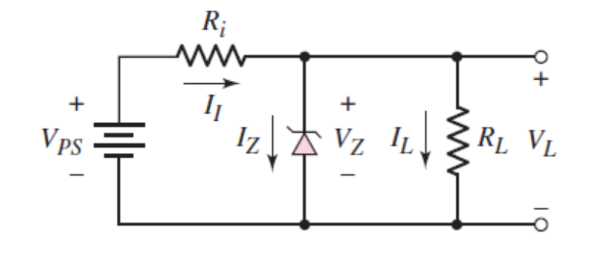
\includegraphics[scale=0.3]{img/p2e.png}
	\caption{Problema 2.}
	\label{p2e}
\end{figure}
Se tienen los siguientes datos: Voltaje de entrada $V_{ps} = 10-14V$, $R_L = 20-100\Omega$, voltaje de diodo zener $V_Z = 5.6V$ y corrientes por el diodo $I_Z (\text{min}) = 0.1 I_Z (\text{max})$. \\\\

Primero, encontramos las corrientes mínima y máxima de carga, sabiendo que la corriente máxima la genera la resistencia mínima y viceversa
	\begin{align*}
		I_L (\text{min}) &= \frac{5.6V}{100\Omega} = 0.056A \\
		I_L (\text{max}) &= \frac{5.6V}{20\Omega} = 0.28A.
	\end{align*}
Entonces, utilizando la ecuación $2.30$ del libro \cite{b1} para encontrar la corriente máxima del diodo
	$$ I_Z (\text{max}) = \frac{I_L (\text{min}) \qty[V_{ps} (\text{max}) - V_Z] - I_L (\text{min}) \qty[V_{ps} (\text{min}) - V_Z]}{V_{ps} (\text{min}) - 0.9V_Z - 0.1V_{ps} (\text{max})}, $$
la cual valuamos con los datos presentados anteriormente, y se tiene
	$$ I_Z (\text{max}) = 0.5865A, $$
por ende
	$$ I_Z (\text{min}) = 0.05865A. $$
Con esto, encontramos la resistencia $R_i$
	$$ R_i = \frac{V_{ps} (\text{min}) - V_Z}{I_Z (\text{min}) + I_L (\text{max})} = \boxed{12.993\Omega} $$
y la potencia mínima del diodo (calculada utilizando la corriente mínima del mismo)
	$$ P_Z (\text{min}) = I_Z (\text{min}) V_Z = \boxed{0.3284W.} $$ \\

\section{Problema 3}
Dado siguiente circuito
\begin{figure}[H]
	\centering
	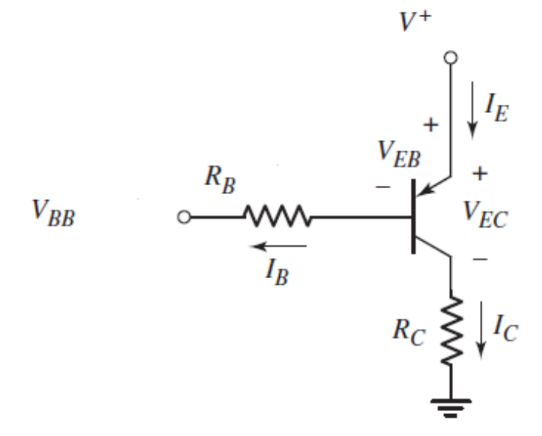
\includegraphics[scale=0.3]{img/p3e.png}
	\caption{Problema 3.}
	\label{p2e}
\end{figure}
con los siguientes datos: $V^+ = 3.3V$, $R_B = 400k\Omega$, $R_C = 5.25k\Omega$, $\beta = 80$, $V_{EB} (\text{on}) = 0.7V$ y $V_{BB} = 1.2V$ (el cual era un dato faltante). \\\\

La corriente $I_B$, la podemos encontrar por ley de nodos de Krichhoff
	$$ I_B = \frac{V^+ - V_{EB} (\text{on}) - V_{BB}}{R_B} = \boxed{3.5\mu A.} $$
Por la relación conocida de las corrientes en un trasistor \textit{pnp}
	$$ I_C = \beta I_B = \boxed{0.28mA.} $$
Y, por ley de voltajes de Kirchhoff
	$$ V_{EC} = V^+ - I_C R_C = \boxed{1.83V.} $$
Para este problema se realizó la simulación en \textit{Multisim Online}
\begin{figure}[H]
	\centering
	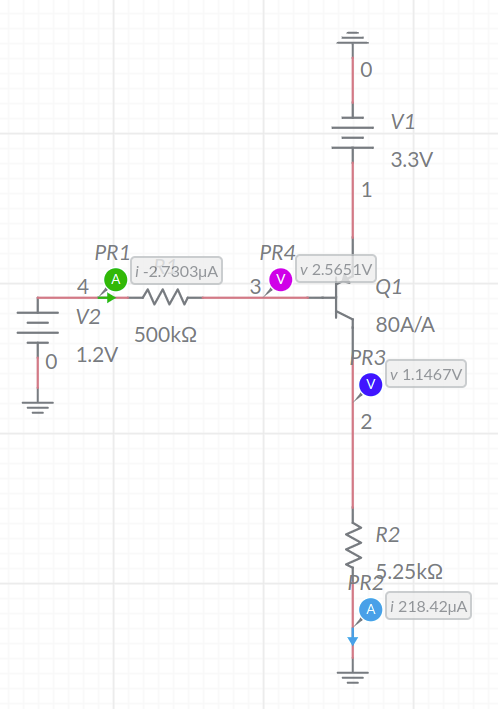
\includegraphics[scale=0.3]{img/p3.png}
	\caption{Problema 3 Simulación.}
	\label{p2e}
\end{figure}
en la cuál podemos analizar varias cosas. Primero era de esperarse que los datos no coicideran completamente con la simulacion, esto debido a que los datos dados en el problema son aproximados; asimismo, los resultados obtenidos son aproximados. Sin embargo, lo obtenido en la simulación es cercano cercano a lo encontrado analíticamente.\\

\section{Problema 4}
Dado el circuito
\begin{figure}[H]
	\centering
	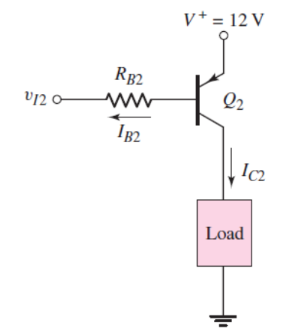
\includegraphics[scale=0.4]{img/p4e.png}
	\caption{Problema 4.}
	\label{p2e}
\end{figure}
Se tienen los siguientes datos: $I_{C2} = 5A$, $\beta = 60$, $V_{EB} (\text{on}) = 0.7V$ y $V_{EC} (\text{sat}) = 0.2V$. \\\\

\begin{enumerate}[a)]
	\item Si se toma $V_{I2} = 12V$, el trasistor se corta y $I_{B2} = I_{C2} = 0$. Pero, si se toma $V_{I2} = 0$, se satura el transistor, entonces $V_{EC} = V_{EC2} (\text{sat}) = 0.2V$, por lo que el voltaje de carga es $V^+ - V_{EC}(\text{sat}) = 11.8V$ y la resistencia de carga sería $R_{\text{Load}} = \flatfrac{11.8V}{5A} = 2.36\Omega$. Para la resitencia $R_{B2}$ asumimos $\flatfrac{I_{C2}}{I_{B2}} = \frac{1}{2} \beta$, entonces $I_{B2} = 0.25A$ y la resistencia
	$$ R_{B2} = \frac{V^+ - V_{EB} (\text{on}) - V_{I2}}{I_{B2}} = \boxed{45.2\Omega .} $$
	\item Para los siguientes datos: $I_{C2} = 2A$, $\flatfrac{I_{C2}}{I_{B2}} = 25$ y $V_I = 0V$. Con lo primero, encontramos $I_{B2} = 0.08A$ y dado que $V_I = 0V$, el transistor se debe saturar, entonces, la resistencia de carga es 
		$$ R_{\text{Load}} = \frac{12 - 0.2V}{2A} = 5.9\Omega .$$
	Y la resistencia $R_{B2}$
		$$ R_{B2} = \frac{V^+ - V_{EB} (\text{on}) - V_{I2}}{I_{B2}} = 141.25\Omega . $$
	Con estos datos se rediseñaría el circuito.
\end{enumerate}





%\begin{abstract}
%    
%\end{abstract}
%
%\begin{IEEEkeywords}
%    
%\end{IEEEkeywords}
%
%\section{Objetivos}
%
%\subsection{General}
%    \begin{enumerate}[1.]
%        \item 
%    \end{enumerate}
%\subsection{Específicos}
%    \begin{enumerate}
%        \item 
%    \end{enumerate}
%%\section{Introducción}
%    
%\section{Marco Teórico}
%    
%\section{Diseño Experimental}
%    \subsection{Materiales a Utilizar}
%        \begin{itemize}
%    	\item 
%    \end{itemize}
%
%    \subsection{Procedimientos}
%        \begin{enumerate}
%            \item 
%        \end{enumerate}
%\section{Resultados}
%    
%\section{Discusión de Resultados}
%\begin{enumerate}
%    \item 
%   
%\end{enumerate}
%\section{Conclusiones}
%\begin{enumerate}
%    \item 
%\end{enumerate}
%%\section{Recomendaciones}
%
%\section{Anexos}
%
\begin{thebibliography}{00}
\bibitem{b1} Neamen, D. A. (2007). \textit{Microelectronics: circuit analysis and design} (Vol. 43). New York: McGraw-Hill.
\end{thebibliography}

\end{document}